\subsection{Monoculture botnets: why the peers must be diverse}
The twelve-device fleet has three instances each of four models. A botnet infects $k$ of the three
SimpleHome XCS7-1003 cameras and poisons all of them together during strong drift
(Figure~\ref{fig:monoculture}; without drift no rule was compromised). Same-model consensus, as in CIoTA~\cite{ciota}, works while the
infected cameras are a minority of their group: with one of three infected it is compromised in
\MonoCiotaOne\ of runs. Once two or three of the three are infected, the consensus \emph{is} the botnet,
and it is compromised in \MonoCiotaThree\ of runs; FOA restricted to same-model peers fails the same way
(\MonoSameThree). FOA with vulnerability-diverse peers is compromised in \MonoFOAThree\ of runs at every
$k$, as is FOA listening to all peers, because one exploit reaches at most three of eleven peers. This
is the head-to-head that separates FOA from same-model consensus. In this fleet, diversity has a cost:
a device whose only diverse peers are three other models gets a coarser consensus and higher false
alarms than one listening to all peers, so in practice a peer group should be as large as possible
subject to no single vulnerability class holding half of it.

\begin{figure}[t]
\centering
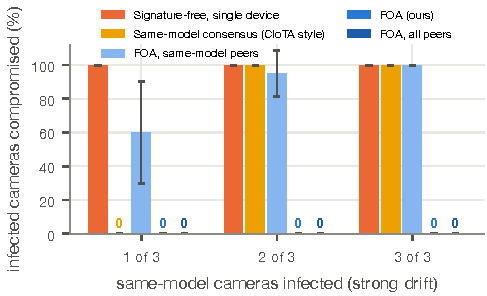
\includegraphics[width=\columnwidth]{figures/fig_monoculture.pdf}
\caption{Monoculture botnet: $k$ of three same-model cameras are infected and poisoned together.
Same-model consensus fails as soon as the infected cameras are a majority of their model; FOA with
diverse peers does not.}
\label{fig:monoculture}
\end{figure}

\subsection{The freeze attack}
An attacker sends loud decoy traffic (real attack packets, pushed out to twice the alarm radius) to one
device from cycle 40 to 100, while strong honest drift runs from cycle 40 to 160, and then leaves
(Figure~\ref{fig:freeze}). Decoys are never learned from by any rule; their only possible effect is on a
stop-learning gate. The alarm-rate switch-off closes as soon as decoys arrive, honest drift moves on
without it, and when the attacker leaves the alarm rate stays high because the traffic has drifted
away: the gate never reopens and the device ends at \KLFrozenFPR\ false alarms, against \KLCleanFPR\
for the same gate without the attacker, at every decoy share from 5\% upward. Not every gate freezes:
the outlier-ratio gate compares the alarm rate with its own moving average, which rises with the decoys,
so it reopened and ended where it would have without the attacker (\ORFrozenFPR); the frozen reserve has
no gate to trip but suffers from the drift itself. FOA's trajectory is unchanged (\FOAFreezeFPR\ with the attacker,
\FOAFreezeClean\ without), exactly as Proposition~\ref{prop:freeze} states; our unit tests check that the
two trajectories are bit-for-bit identical.

\begin{figure*}[t]
\centering
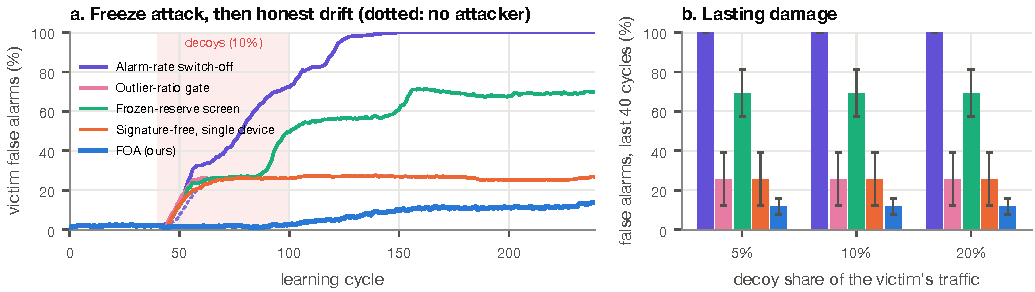
\includegraphics[width=\textwidth]{figures/fig_freeze.pdf}
\caption{Freeze attack. (a) False alarms on the targeted device; decoys from cycle 40 to 100 (10\% share),
honest drift from 40 to 160. Dotted: same rule, no attacker. (b) False alarms over the last 40 cycles
by decoy share.}
\label{fig:freeze}
\end{figure*}

\subsection{Attacks on the gossip}
\textbf{Byzantine peers.} With strong drift, FOA is not compromised with one or two of the victim's
seven peers fully controlled by the attacker (\ByzO, \ByzT), but it is with three (\ByzH), although three
of seven is below the geometric median's breakdown point. This is Theorem~\ref{thm:byz}'s caveat in
practice: during drift the victim agrees with the consensus, so a consistent bias of order $C_\alpha r$
per cycle is applied, and our default common budget is generous enough to let it accumulate. Without
drift the victim's own traffic does not back the biased consensus and no number of Byzantine peers
compromised it. A tighter common budget would trade shared-drift liveness for this case.
\textbf{Keyless attackers.} Twelve forged frames per cycle plus replays of the previous cycle's frames
had no effect (\SybilFOA\ compromised; every forged and replayed frame was rejected). With
authentication switched off, the same attacker compromised the victim in \SybilNoHMAC\ of runs.
\textbf{Lossy radio.} Losing up to 70\% of frames changed little (fleet false alarms \LossNoneFPR\
with no loss, \LossHalfFPR\ at 50\%); at 90\% most cycles have fewer than two peers, FOA falls back to
its residual budget and false alarms rise.

\begin{figure*}[t]
\centering
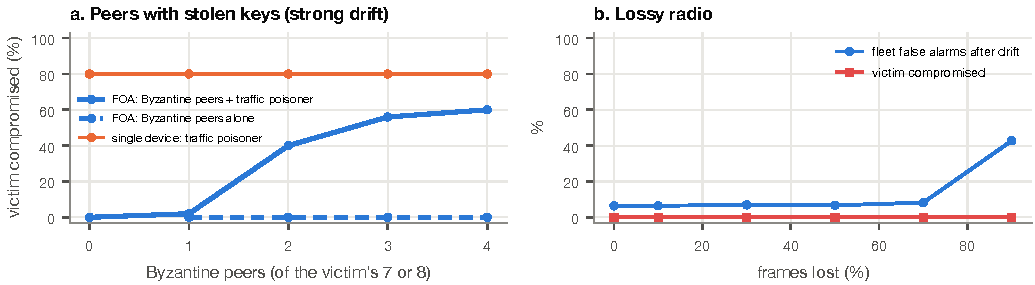
\includegraphics[width=0.8\textwidth]{figures/fig_gossip.pdf}
\caption{Attacks on the gossip. (a) Byzantine peers with valid keys. (b) Frame loss.}
\label{fig:gossip}
\end{figure*}

\subsection{One knob: the residual rate}\label{sec:frontier}
Table~\ref{tab:sweep} sweeps $B$. With $B\le$\SweepSafeMaxB\ alarm radii per cycle no victim was
compromised; larger $B$ admits the attacker faster (\SweepCompHigh\ compromised at $B=0.04$). In
exchange, a device's own drift is followed faster: false alarms after device-only drift fall from
\SweepIdioLow\ at the smallest $B$ to \SweepIdioHigh\ at $B=0.02$. No setting is free, as
Proposition~\ref{prop:frontier} says; the bound of Corollary~\ref{cor:ttc} held in every run of the
sweep (\SweepViol\ violations). Figure~\ref{fig:theory} repeats the sweep on a synthetic fleet with known
geometry and checks the Byzantine lemma numerically.

\begin{figure*}[t]
\centering
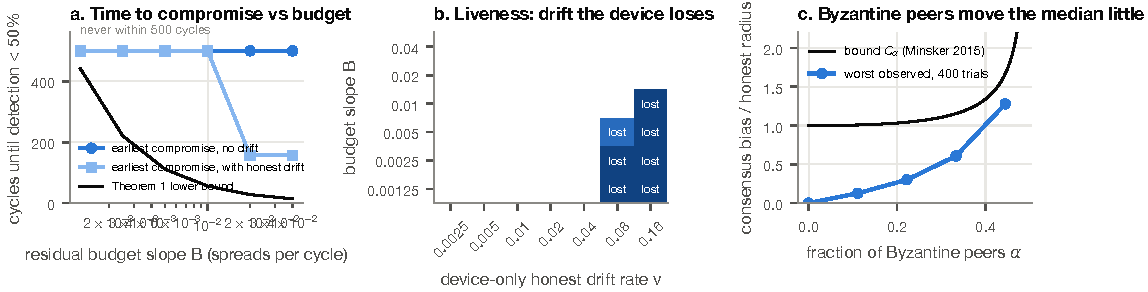
\includegraphics[width=\textwidth]{figures/fig_theory.pdf}
\caption{Theory checks on a synthetic fleet with known geometry. (a) Earliest compromise against the
budget slope, with the closed-form lower bound of Corollary~\ref{cor:ttc}. (b) Device-only drift rates
that a device loses, for each budget slope. (c) Worst observed consensus bias with $f$ Byzantine peers
against Lemma~\ref{lem:gm}.}
\label{fig:theory}
\end{figure*}

\subsection{Ablations and adaptive attackers}\label{sec:ablation}
Table~\ref{tab:ablation} removes one piece at a time. Discarding the residual instead of rationing it
(the CIoTA choice applied to diverse peers) leaves devices unable to follow anything their peers do not
share: fleet false alarms rise to \AblDiscardFPR. Removing the peers (budget only) gives
\AblNoPeersFPR. Removing the residual budget gives back the attack (\AblFullComp\ compromised). Measuring
agreement with a mean instead of a median roughly doubles false alarms (\AblMeanLamFPR\ against
\AblFOAFPR), because an attacker can then cancel the victim's agreement and stall it. A wider spread
budget or a joint centre-and-spread budget lets attackers through: inflating the spread is the cheapest
way to make an attack fit. When a device has its own large drift on top of the shared one, almost every
variant loses that device (false alarms of 74 to 100\%); only the variants with more room (no residual
budget, or one joint budget) partly keep up, and both are poisoned. Removing the residual budget is also
the only change that ever violated the bound of Corollary~\ref{cor:ttc} (4 runs), as it should. Among
adaptive attackers (strong drift, share 0.3, three victims), pulsing compromised no one under either
rule; FOA cut the core-hiding attacker from 33\% to 10\%; and multi-direction, consensus-aligned and
mimicry attackers each compromised one of the three victims (33\%) under both FOA and single-device
adaptation, so FOA did not help against them on that victim.

\subsection{A four-node fleet}
The testbed has four ESP32 nodes. Simulating a fleet of four vendors (Danmini, Ecobee, Provision PT-838,
SimpleHome XCS7-1003) with strong drift and a boundary attacker at share 0.3: FOA \FourCompFOA\
compromised with \FourFPRFOA\ fleet false alarms; single-device adaptation \FourCompAuto\ and
\FourFPRAuto; alarm-rate switch-off \FourCompKL\ and \FourFPRKL; frozen reserve \FourCompFrozen\ and
\FourFPRFrozen. Three peers are enough for the consensus to work. Joining devices were never
compromised in our join experiment (\JoinComp), with or without the warm start.

\subsection{Real drift: 40 weeks of CESNET traffic}\label{sec:cesnet}
The injected drift above is a stress test. To check FOA on drift nobody designed, we use
CESNET-TimeSeries24~\cite{cesnet}: traffic statistics of IP addresses in a national research network
from October 2023 to July 2024, which span a semester, holidays and the institutions' own changes. The
fleet is the twelve most active addresses of one institution (they share its network); a learning cycle
is one day of 10-minute aggregates (twelve statistics: flows, packets, bytes, destinations, ports,
protocol and direction ratios, duration, TTL), the first 28 days calibrate, and 252 days stream. Nothing
about the drift is injected. The attack is modelled, because the dataset has no attack labels: the IP's
own traffic turned into a scanner (twenty times the flows, thirty times the destinations, short flows),
with a boundary poisoner from day 30. Eleven of the twelve addresses meet the victim rule.

The real drift is milder than our stress test: the static detector stays at \CesStaticFPR\ false
alarms, except one address whose behaviour changes for good in the second half and which every rule
loses. Every adaptive rule pays something for adapting to daily variation (single device \CesAutoFPR,
alarm-rate switch-off \CesKLFPR); FOA pays least among the protected rules (\CesFOAFPR). Under attack,
naive learning was compromised in \CesNaiveComp\ of runs, single-device adaptation and the alarm-rate
switch-off in \CesAutoComp\ and \CesKLComp, the frozen reserve in \CesFrozenComp, and FOA in
\CesFOAComp\ (Figure~\ref{fig:cesnet}).

\begin{figure*}[t]
\centering
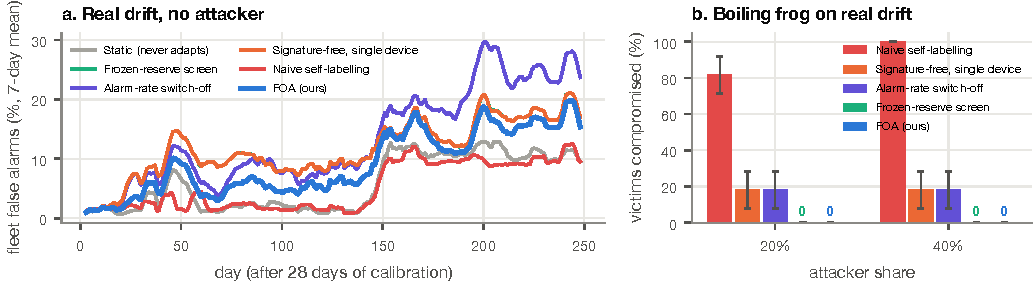
\includegraphics[width=\textwidth]{figures/fig_cesnet.pdf}
\caption{CESNET-TimeSeries24, twelve addresses of one institution, one learning cycle per day.
(a) Fleet false alarms under real drift, no attacker (the frozen reserve never filters here and coincides with single-device adaptation). (b) Victims compromised by a boundary poisoner
(11 victims, 5 held-out seeds).}
\label{fig:cesnet}
\end{figure*}

